\chapter{Evaluation}
This chapter critically examines the machine learning models conceived and partially implemented in the previous chapter.
Table X shows an overview of the evaluated criteria. These are structured according to the Goal-Question-Metric approach

Mean Absolute Error (MAE)
how far the predictions are from the actual output


\begin{longtable}{|l|p{6cm}|p{3cm}|}
    \hline
    \textbf{Goal}                 & \textbf{Question}                                                                                               & \textbf{Metric}                                      \\

    \hline
    \textbf{Appropriatness}       & How well does the model type fit the current task?                                                              & Prerequisites for model type                         \\
    \hline
    \textbf{Correctness}          & Ability of the model to perform the current task measured on the development dataset and the runtime dataset    &
    Precision, Recall, F-score                                                                                                                                                                             \\
    \hline
    \textbf{Relevance}            & Does the model achieve a good bias-variance tradeoff? Which means neither overfitting or unterfitting the data. & Variance of cross-validation and fit                 \\
    \hline
    \textbf{Robustness}           & Ability of the model to outliers, noise and other data quality issues                                           & Variance of cross-validation, fit                    \\
    \hline
    \textbf{Stability}            & Does the artifact generate repeatable results when trained on different data?                                   & Equalized Loss of Accuracy (ELA)                     \\
    \hline
    \textbf{Interpretability}     & How well can the model be explained?                                                                            & Complexity measures (e.g., no. of parameters, depth) \\
    \hline
    \textbf{Resource utilization} & How much resources are required to train and run the model?                                                     & Training time, runtime, storage space                \\
    \hline
    \caption{Overview of the goals, questions and metrics for the evaluation of artifacts following the \ac{GQM} approach.}
\end{longtable}

\section{Correctness}
\subsection{Random Forest} 
With 100 estimators in \ac{RF} a \ac{mse} of 0.15 and \ac{rmse} 0.39 was achieved. 
Figure~\ref{fig:rf_feature_importance} compares and visualizes the relative importance of the features used for training the model. 
As shown, the thickness is the most important feature followed by distance and die open. The results show, that all three featured are relevant for the outcome and so no feature can be removed from the dataset to get a better performance of the model. 


\begin{figure}[H]
    \centering
    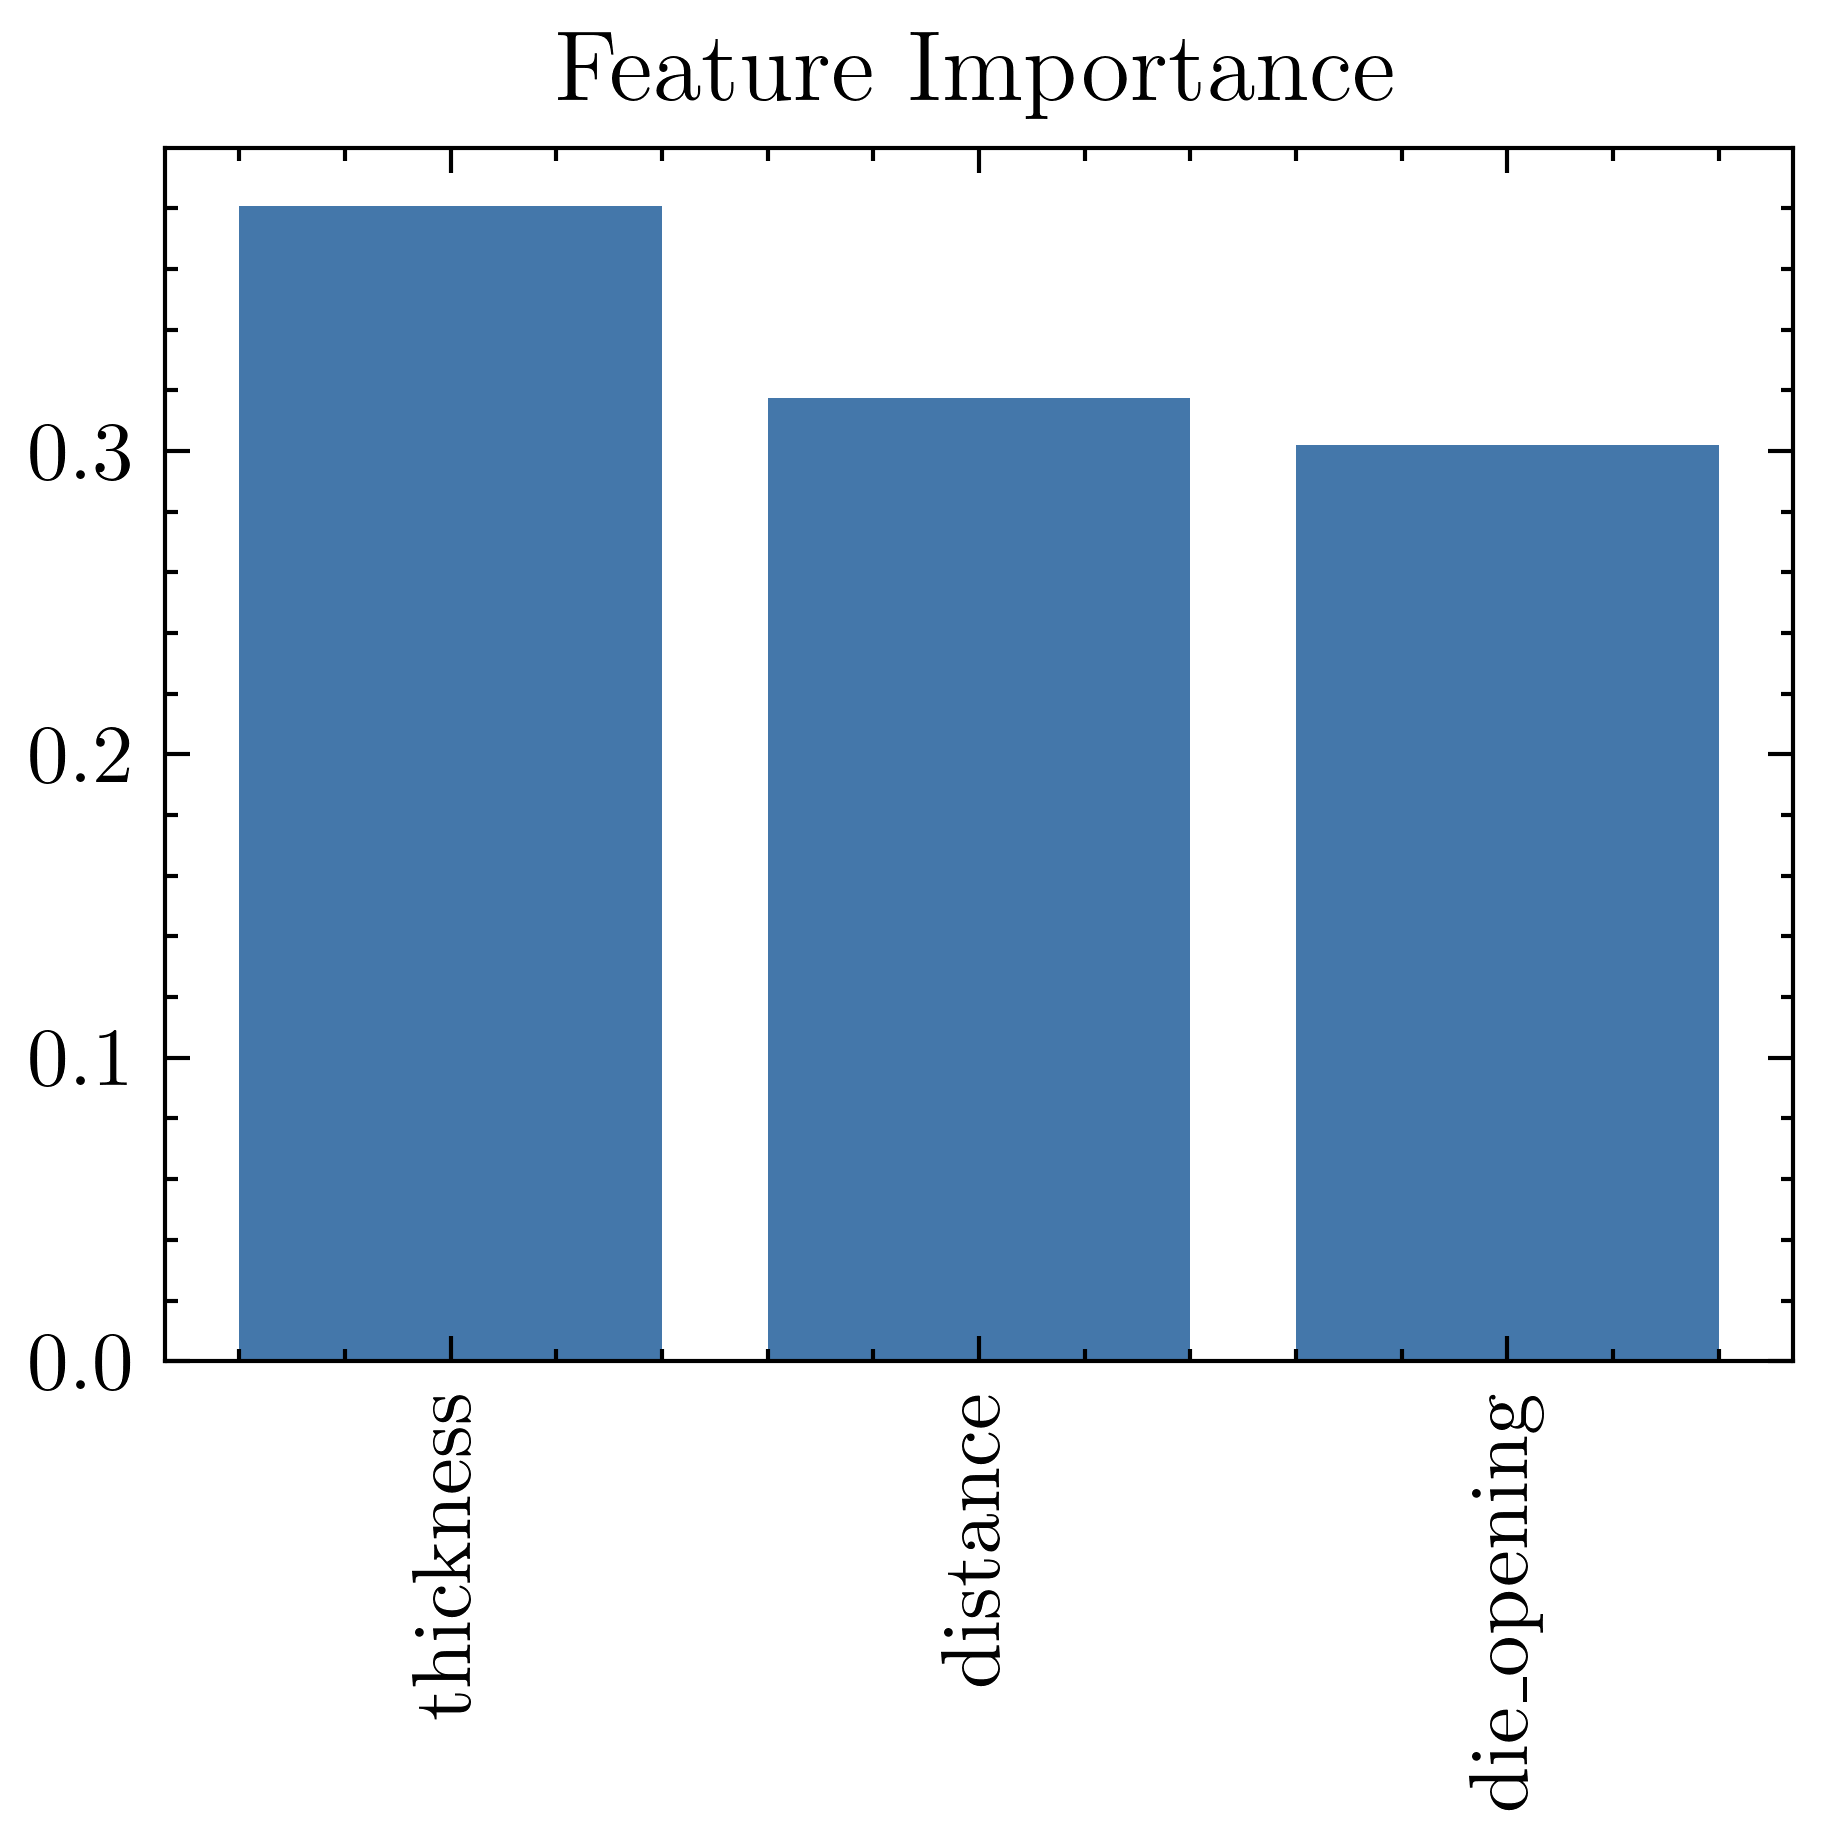
\includegraphics[width=0.6\textwidth]{Random_Forest_Regression_importances}
    \caption{Relative feature importance}
    \label{fig:rf_feature_importance}
\end{figure}

In further experiments boosting was used with the goal of predicting the target vector more precise. A \ac{mse} of 0.27 and \ac{rmse} of 0.52 as achieved and therefore no better performance to the default random forest. 








\section{Summary}